%%%%%%%%%%%%%%%%%%%%%%%%%%%%%%%%%%%%%%%%%
% University/School Laboratory Report
% LaTeX Template
% Version 3.1 (25/3/14)
%
% This template has been downloaded from:
% http://www.LaTeXTemplates.com
%
% Original author:
% Linux and Unix Users Group at Virginia Tech Wiki 
% (https://vtluug.org/wiki/Example_LaTeX_chem_lab_report)
%
% License:
% CC BY-NC-SA 3.0 (http://creativecommons.org/licenses/by-nc-sa/3.0/)
%
%%%%%%%%%%%%%%%%%%%%%%%%%%%%%%%%%%%%%%%%%

%----------------------------------------------------------------------------------------
%	PACKAGES AND DOCUMENT CONFIGURATIONS
%----------------------------------------------------------------------------------------

\documentclass{article}

\usepackage[version=3]{mhchem} % Package for chemical equation typesetting
\usepackage{siunitx} % Provides the \SI{}{} and \si{} command for typesetting SI units
\usepackage{graphicx} % Required for the inclusion of images
\usepackage{natbib} % Required to change bibliography style to APA
\usepackage{amsmath} % Required for some math elements 
\usepackage{enumerate} % Required for the enumerate function
\usepackage[siunitx]{circuitikz} % Required for the drawing of circuit diagrams
\usepackage{caption}
\usepackage{graphicx}
\usepackage{subcaption}
\usepackage{xfrac}
\usepackage{float}
\usepackage{enumitem}
\usepackage{chemgreek}
\usepackage{epstopdf}


\setlength\parindent{0pt} % Removes all indentation from paragraphs

\renewcommand{\labelenumi}{\alph{enumi}.} % Make numbering in the enumerate environment by letter rather than number (e.g. section 6)

%\usepackage{times} % Uncomment to use the Times New Roman font

\graphicspath{{./fig/}}

%----------------------------------------------------------------------------------------
%	DOCUMENT INFORMATION
%----------------------------------------------------------------------------------------

\title{Electrical Machines \& Power Systems \\ Practical 2 - Three Phase Induction Motors \\ ENG224} % Title

\author{Shane \textsc{Reynolds}} % Author name

\date{October 1, 2016} % Date for the report

\begin{document}

\maketitle % Insert the title, author and date

\begin{center}
\begin{tabular}{l r}
Date Performed: & September 09, 2016 \\ % Date the experiment was performed
Instructor: & Dr Kamal Debnath % Instructor/supervisor
\end{tabular}
\end{center}

% If you wish to include an abstract, uncomment the lines below
% \begin{abstract}
% Abstract text
% \end{abstract}

%----------------------------------------------------------------------------------------
%	SECTION 1
%----------------------------------------------------------------------------------------

\section{Objective}

To find, experimentally, the circuit parameters of the equivalent circuit for a three phase induction motor, and provide predictions of the motor performance. The induction motor is a 4 pole squirrel cage asynchronous motor which is applied to a balanced three phase power source. 
 
%----------------------------------------------------------------------------------------
%	SECTION 2
%----------------------------------------------------------------------------------------

\section{Procedure and Results}
\subsection{Direct on line (DOL) starting}
Direct on line starting applies the motor terminals directly to the full line voltage. In this instance the stator was connected in a delta configuration, which was then connected to a voltage source equal to the rating of the stator windings of the motor (240$\si{\volt}$). The motor was switched on and the observed starting current was 0.75$\si{\ampere}$. The rated line current was 0.7$\si{\ampere}$. This method of starting 

\subsection{Reduced voltage starting}
In the previous section, it was seen that the current using a DOL starter draws a high inrush current in excess of the rated line current. To overcome this issue, a star-delta starter might be used. This is a physical switch which has connections both in star and delta configurations. On start up of the 4 pole squirrel cage induction motor, the motor is originally in a star configuration with the power source, and once up to speed, is switched to a delta configuration. A circuit schematic of a start-delta starter can be seen in Figure 1.

\begin{figure}[H]
	\begin{circuitikz}
		\draw (0,0)
		to [switch,o-](2,0)
		to [short](3,0)
		to [short](3,-2)
		to [short] (6,-2)
		to [L,l_=$RR^1$] (8,-2)
		to [short] (9,-2)
		to [short] (9,-1.5)
		to [short] (6,-1.5)
		to [short] (6,2)
		to [short] (7,2)
		to [switch,] (8,2)
		;
		
		\draw (0,-1)
		to [switch,o-](2,-1)
		to [short](2.5,-1)
		to [short](2.5,-3)
		to [short](6,-3)
		to [L,l_=$YY^1$] (8,-3)
		to [short] (9.5,-3)
		to [short] (9.5,-1)
		to [short] (6.5,-1)
		to [short] (6.5,1)
		to [short] (7,1)
		to [switch] (8,1)
		;
		
		\draw (0,-2)
		to [switch,o-](2,-2)
		to [short] (2,-4)
		to [short] (6,-4)
		to [L,l_=$BB^1$] (8,-4)
		to [short] (10,-4)
		to [short] (10,-0.5)
		to [short] (7,-0.5)
		to [short] (7,0)
		to [switch] (8,0)
		to [short] (8,2)
		;
		
		\draw (5,-2)
		to [short,*-] (5,0.5)
		to [short,-*] (7.5,0.5)
		;
		
		\draw (4.5,-4)
		to [short,*-] (4.5,1.5)
		to [short,-*] (7.5,1.5)
		;
		
		\draw (4,-3)
		to [short,*-] (4,2.5)
		to [short,-*] (7.5,2.5)
		;
		
		\draw (9,2) to [short,l=$R^1$] (9,2);
		\draw (9,1) to [short,l=$Y^1$] (9,1);
		\draw (9,0) to [short,l=$B^1$] (9,0);
		
		\draw (-0.5,0) to [short,l=$R$] (-0.5,0);
		\draw (-0.5,-1) to [short,l=$Y$] (-0.5,-1);
		\draw (-0.5,-2) to [short,l=$B$] (-0.5,-2);
	\end{circuitikz}
	\caption{The circuit schematics for a star-delta starter. There are two banks of switches: one set to connect the three phase power, and the second bank to change from star to delta.}
\end{figure}

The induction motor, was started with this method and an output a starting current of 0.6$\si{\ampere}$ was recorded. Theory dictates that the starting current should fall to approximately two thirds of the starting current observed in DOL. The experimental evidence obtained shows that the drop was only about a quarter of the DOL current.

\subsection{No load test}
The no load test is similar in nature to the open circuit test on a transformer. The test is performed by applying a balanced rated voltage on the stator windings. The equivalent circuit for the induction motor can be seen in Figure 2.

\begin{figure}[H]
	\centering
	\ctikzset{bipoles/length=0.8cm}
	\begin{circuitikz}
		\draw
		(0,2) 
		to [short,i=$I_{NL}$,o-](2,2)
		to[R,l=$R_1 + R'_2$] (4,2)
		to[L,l=$X_1 + X'_2$] (6,2) 
		to[R, l=$\frac{1-s}{s} \cdot R'_2$] (6,0)
		to[short,-o] (0,0)
		;
		\draw
		(1.5,2) to [short,i=$I_{\phi}$](1.5,1.5) -- (1,1.5)
		to[R,l_=$R_C$,i_=$I_C$](1,0);
		\draw
		(1.5,1.5) -- (2,1.5)
		to[L,l=$X_m$,i=$I_m$](2,0)
		;
		\draw (0,1) to [short,l=$V_{rated}$](0,1);
	\end{circuitikz}
	\caption{Equivalent circuit for the induction motor described in the problem.}
\end{figure}

In the even of no load, the machine will rotate at almost synchronous speed which means the slip is nearly zero. In this instance, we get an open circuit across $\big( \sfrac{(1-s)}{s} \big) \cdot R'_2$ - this results in an equivalent circuit like that shown in Figure 3.

\begin{figure}[H]
	\centering
	\ctikzset{bipoles/length=0.8cm}
	\begin{circuitikz}
		\draw
		(-1,2) 
		to [short,i=$I_{NL}$,o-](1.5,2)
		;
		\draw
		(1.5,2) to [short,i=$I_{\phi}$](1.5,1.5) -- (1,1.5)
		to[R,l_=$R_C$,i_=$I_C$](1,0)
		to[short](1.5,0)
		;
		\draw
		(1.5,1.5) -- (2,1.5)
		to[L,l=$X_m$,i=$I_m$](2,0)
		to[short](1.5,0)
		to[short](1.5,-0.5)
		to[short,-o] (-1,-0.5)
		;
		\draw (-1,0.75) to [short,l=$V_{rated}$](-1,0.75);
	\end{circuitikz}
	\caption{Equivalent circuit for the induction under a no load test.}
\end{figure}

The supply voltage was increased to the rated voltage of $240\si{\volt}$, and the following values were recorded:
\begin{center}
	\fbox{	Input Power = $18\si{\watt}$ \ \ Current = $0.1\si{\ampere}$ \ \ Speed = $1495 \ \si{rpm}$}
\end{center}

Using these experimental values, estimates for both $R_C$ and $X_m$ can be found. First, we know that the power $P_{NL}$ can be found using the following expression:
\begin{align*}
	P_{NL} = 3 \cdot V_{rated} \cdot I_{NL}
\end{align*}

Rearranging, and using Ohm's law, we arrived at the following expression for $R_C$:
\begin{align*}
	R_C &= \frac{3 \cdot V_{rated}^2}{P_{NL}}\\
		&= \frac{3 \times 240^2}{18}\\
		&= 9600 \si{\ohm}
\end{align*}

Hence, we see that:
\begin{center}
	\fbox{$R_C = 9.6\si{\kilo\ohm}$}
\end{center}
\vspace{0.5cm}
We can now find $I_C$, again, using Ohm's law:
\begin{align*}
	I_C = \frac{V_{rated}}{R_C} = \frac{240}{9600} = 0.025\si{\ampere}
\end{align*}

Using the fact that the current through the induction shunt is orthogonal to the current through the resistive shunt, we can find $I_m$:
\begin{align*}
	I_m &= \big(I_{NL}^2 - I_C^2\big)^{\sfrac{1}{2}}\\
		&= \bigg(\big(\frac{0.1}{\sqrt{3}}\big)^2 - 0.025^2 \bigg)^{\sfrac{1}{2}}\\
		&= 0.0520\si{\ampere}
\end{align*}

Finally, we can find $X_m$ as follows:
\begin{align*}
	X_m = \frac{V_{rated}}{I_m} = \frac{240}{0.0968} = 4615.38\si{\ohm}
\end{align*}

Hence, we have that:
\begin{center}
	\fbox{$X_m = 4615.38\si{\ohm}$}
\end{center}
\vspace{0.5cm}
The slip in this scenario can be found as:
\begin{align*}
	s = \frac{n_s - n}{n} = \frac{1500 - 1495}{1495} = 0.0033
\end{align*}

As predicted, the machine is almost running at synchronous speed with a slip:
\begin{center}
	\fbox{$s = 0.33\%$}
\end{center}

\subsection{Locked rotor test}
The locked rotor test for an asynchronous induction motor is similar in nature to the short circuit test on a transformer. A mechanical device stops the rotor from turning, and low voltage is applied to the stator windings until the rated current is recorded. In this instance we note that there is no rotation slip, $s=1$. Hence, the full equivalent circuit seen in Figure 2 will simplify to that seen in Figure 4.

\begin{figure}[H]
	\centering
	\ctikzset{bipoles/length=0.8cm}
	\begin{circuitikz}
		\draw
		(0,2) 
		to [short,i=$I_{rated}$,o-](2,2)
		to[R,l=$R_1 + R'_2$] (4,2)
		to[L,l=$X_1 + X'_2$] (6,2) 
		to[short] (6,0)
		to[short,-o] (0,0)
		;
		\draw (0,1) to [short,l=$V_{LR}$](0,1);
	\end{circuitikz}
	\caption{Equivalent circuit for the induction motor described in the problem.}
\end{figure}

The supply voltage was increased until the current reached the rated stator current of $0.7\si{\ampere}$, and the following values were recorded:
\begin{center}
	\fbox{	Input Power = $140\si{\watt}$ \ \ Voltage = $171.70\si{\volt}$ }
\end{center}
\vspace{0.5cm}
Now, we can find $R_eq$ using the power relationship $P_{sc} = 3 \cdot V_{LR} \cdot I_{LR}$. Rearranging we get that:
\begin{align*}
	R_{eq} = \frac{P_{sc}}{3 \cdot I_{LR}^2} = \frac{140}{3 \cdot \big(\frac{0.7}{\sqrt{3}}\big)^2} = 285.71\si{\ohm}
\end{align*}

We can find the impedence of the equivalent circuit using Ohm's law:
\begin{align*}
	Z_{eq} = \frac{V_{LR}}{I_{LR}} = \frac{171.27}{\frac{0.7}{\sqrt{3}}} = 427.32\si{\ohm}
\end{align*}

Hence, since resistance and reactance are orthogonal, we can find the reactance as follows:
\begin{align*}
	X_{eq} = \sqrt{Z_{eq}^2 - R_{eq}^2} = \sqrt{427.32^2 - 285.71^2} = 317.77\si{\ohm}
\end{align*}

Hence, the parameters $R_{eq}$ and $X_{eq}$ are as follows:
\begin{align*}
	\fbox{$R_{eq} = 285.71\si{\ohm} \quad X_{eq} = 317.77\si{\ohm}$}
\end{align*}

\subsection{Stator resistance}
The stator resistance was measured simply using a digital multimeter. The stator resistance is as follows:
\begin{center}
	\fbox{$R_1 = 47.90\si{\ohm}$}
\end{center}

\subsection{Equivalent circuit parameters and predicted performance}

To find the torque-speed characteristic equation, we need to first find a value for $R'_2$. We note that $R_{eq} = R_1 + R'_2$. Hence, we see that:
\begin{align*}
	R'_2 = R_{eq} - R_1 = 285.71 - 47.90 = 236.71\si{\ohm}
\end{align*}

Now, the torque-speed characteristic equation is given by:
\begin{align*}
	T_{mech} = \frac{1}{\omega_{sync}} \cdot \bigg[\frac{V_1}{\big(R_1 + \frac{R'_2}{s}\big)^2 + \big(X_1 + X'_2\big)^2}\bigg] \cdot \frac{R'_2}{s}
\end{align*}

Now, we can find $\omega_{sync}$ using the following:
\begin{align*}
	\omega_{sync} = n_{sync} \cdot \frac{2 \pi}{60} = 1500 \cdot \frac{2 \pi}{60} = 157.07\si{\radian\per\second}
\end{align*}

Hence, the torque-speed characteristic equation is given by:
\begin{center}
	\fbox{$T_{mech} = \frac{1}{157.07} \cdot \bigg[\frac{240}{\big(47.90 + \frac{236.71}{s}\big)^2 + 317.77^2}\bigg] \cdot \frac{236.71}{s}$}
\end{center}

\begin{figure}[H]
	\centering
	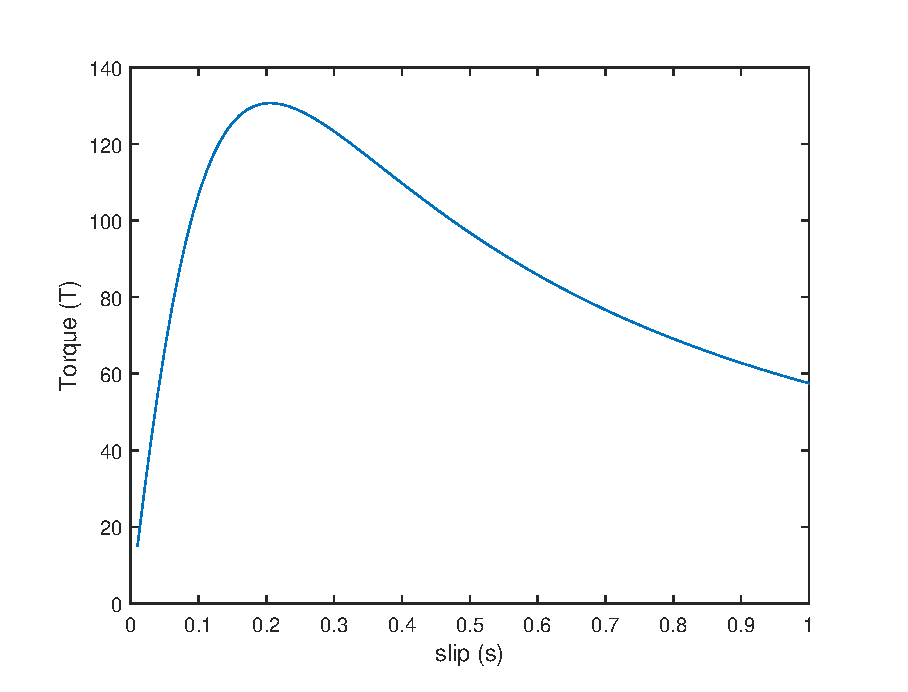
\includegraphics[scale=0.5]{fig2}
	\caption{Plot of the torque-speed characteristic equation, with $s_{T_{max}} = 0.174$}
\end{figure}

A plot of the torque-slip characteristic equation can be seen in Figure 5. Finally, the slip at which maximum torque occurs is given by:
\begin{align*}
	s_{T_{max}} = \frac{(R'_2)^2}{\sqrt{R_1^2 + X_{eq}^2}} = \frac{236.71^2}{\sqrt{47.90^2 + 317.77^2}} = 0.2
\end{align*}

The slip at which the maximum torque occurs is given by:
\begin{center}
	\fbox{$s_{T_{max}} = 0.174$}
\end{center}


%----------------------------------------------------------------------------------------
%	SECTION 4
%----------------------------------------------------------------------------------------

\section{Conclusions}
Equivalent circuit parameters of a three phase induction motor were found using the no load and short circuit tests. The following parameters were found:
\begin{align*}
	R_C &= 9.6\si{\kilo\ohm}\\
	X_m &= 4615.38\si{\ohm}\\
	R_1 &= 47.90\si{\ohm}\\
	R'_2 &= 236.71\si{\ohm}\\
	s_{T_{max}} &= 0.174
\end{align*}

\end{document}